
\PassOptionsToPackage{unicode}{hyperref}
\PassOptionsToPackage{naturalnames}{hyperref}
\documentclass{beamer} 
%\usepackage{babel}
%\usepackage[utf8]{inputenc}


%%% FONT SELECTION %%%%%%%%%%%%%%%%%
%%% we choose a sans font %%%%%%%%%%
\usepackage{kmath,kerkis} 
%\usepackage[default]{gfsneohellenic} 
%%%%%%%%%%%%%%%%%%%%%%%%%%%%%%%%%%%%

\usepackage{color}
\usepackage{amsmath}
\usepackage{amssymb}

\usepackage{epstopdf}
\usepackage{graphicx}
\graphicspath{{./images/presentation}}

%%
% load TEI-Pel - specific layout
\usepackage{TeiPel_En_Beamer_Layout}
\setTeipelLayout{draft,newlogo}% options: "draft", "newlogo"
















% Thesis Info - first page 
	% title
		\title[This is my Title]{Presentation\\ Title}	
	% author 
    % (In the mandatory argument "{}", separate multiple
    % authors with "\and" - use "\\" for better author name formatting
    % in the title page. In the optional argument "[]" include all
	% author names, with no "\and" or text formatting macros.)
	% Example: 
    %\author[A. Author Albert Einstein]{Anthony Author \and Albert Einstein}
		\author[A. Author]{Anthony Author}
	% supervisor	
		\supervisor{Supervisor}{Mister Supervisor}{Professor}
	% date
		\presentationDate{October 22, 2017}


\begin{document}

% typeset front slides
	\typesetFrontSlides

% Your Slides Start here:

\section{Motivaton}

\subsection[Basic Problem]{The basic problem that we have studed}

\begin{frame}{Slide Title \#1}
	\framesubtitle{Slide subtitle \#1}
	\begin{itemize}
		\item Use the \texttt{itemize} environment frequently.
		\pause
		\item Use short sentences and phrases.
		\pause
		\item In this presentation we use the \textbackslash{}\texttt{pause} macro.
	\end{itemize}
\end{frame}

\begin{frame}{Slide Title \#2}
	\begin{itemize}
		\item <1->You can define the order of appearance.
		\item <3->Like here.
		\item <2->This is the second item to appear.
	\end{itemize}
\end{frame}

\begin{frame}{Slide Title \#3}
	\begin{block}
		<1->{}
		\begin{itemize}
			\item Group without title.
			\item Appears for all slides.
		\end{itemize}
	\end{block}
	\begin{exampleblock}
		<2->{Group title}
		\begin{itemize}
			\item $e^{i\pi}=-1$.
			\item $e^{i\pi/2}=i$.
		\end{itemize}
	\end{exampleblock}
\end{frame}

%%
\subsection{Previous work}

\begin{frame}{Slide Title \#4}
	\begin{example}
		<1->First example. 
	\end{example}
	\begin{example}
		<2->Second example.
	\end{example}
\end{frame}

\begin{frame}{Slide Title \#5}
	\begin{center}
		Table example \\[12pt]
		\begin{tabular}{c||c|c|c|}
			& \textbf{col 1} & \textbf{col  2} & \textbf{col 3} \\
			\hline
			\hline
			\textbf{row 1} & 11 & 12 & 13 \\
			\hline
			\textbf{row 2} & 21 & 22 & 23 \\
		\end{tabular}
    \end{center}
\end{frame}

\begin{frame}{Slide Title \#6}
	\begin{center}
		Figure example \\[12pt]
		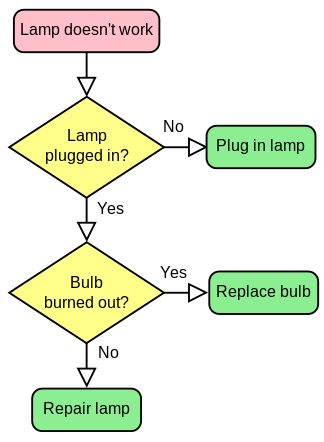
\includegraphics[width=0.35\textwidth,keepaspectratio]{LampFlowchart.png}
		\\
		\footnotesize(source: \textlatin{Wikipedia})
    \end{center}
\end{frame}

\begin{frame}{Slide Title \#7}
	\centering
	Math examples \\[12pt]
	\begin{equation}
        	B'=-\nabla \times E
	\end{equation}
	\begin{equation*}
        	E'=\nabla \times B - 4\pi j
	\end{equation*}
\end{frame}

%%%%
\section{Results / contribution}

%%
\subsection{Main results}

\begin{frame}{Summary}
   	\begin{alertblock}{Attention}
   		\textlatin{This is an important alert}
   	\end{alertblock}
\end{frame}

%
\subsection{Subsection title}

\begin{frame}{Summary}
	\begin{itemize}
		\item The \textcolor{red}{first main message} of our talk.
		\item The \textcolor{red}{second main message} of our talk.
		\item Maybe a \textcolor{red}{third message}, but ... no more.
	\end{itemize}
	\vskip0pt plus.5fill
	\begin{itemize}
		\item Conclusion.
	\end{itemize}
	\begin{itemize}
		\item Future work.
		\item Discussion.
	\end{itemize}
\end{frame}

\begin{frame}{References}
	\begin{thebibliography}{2}
		\beamertemplatebookbibitems
		\bibitem{Author1990}A.\ Author. \newblock\emph{Handbook of Everything}.\newblock
\textlatin{Some Press, \oldstylenums{1990}}.

		\beamertemplatearticlebibitems
		\bibitem{Someone2002}B.\ Author.\newblock On this and that\emph{.}
\newblock\emph{Journal on This and That}. 
\oldstylenums{2}(\oldstylenums{1}):\oldstylenums{50}--\oldstylenums{100}, 
\oldstylenums{2000}.
	\end{thebibliography}
\end{frame}

%%
\end{document}